% ===== INICIO DEL PREÁMBULO =====
%
\documentclass[msc,oneside,a4paper]{udelar} % Poner msc para Maestría, dsc para Doctorado.
%
\usepackage[
acronyms, %utiliza el glosario de acronimos.
nohypertypes={acronym,notacion,simbolos,glosario}, %quita los links en el texto al glosario.
%nonumberlist,                                       %quita los links en los glosarios al texto.
nogroupskip, %quita los espacios entre diferentes grupos dentro de un glosario.
nopostdot, %quita el punto final en los acrónimos
]{glossaries}

\hypersetup{colorlinks=false} % Hipervínculos: escribir "false" para imprimir o "true" para ver en digital.

% Ver los documentos de estilos bibliográficos para editar estas siguientes 2 líneas. Se deben de copiar a partir de los PDF de estilos bibliográficos y no es necesario que el estudiante las edite.
\usepackage{natbib} % Para algunos estilos bibliográficos
\bibliographystyle{estilos_bibliograficos/natbib/apalike}

\loadglossary 

% A su vez, la clase udelar.cls ya tiene los siguientes paquetes cargados automáticamente, que podrían ser de interés saber para el usuario:
% 
% {color},{hyphenat},{appendix},{lastpage},{babel},{inputenc},{amsmath,amssymb},{ifthen},{graphicx},{caption}
% {setspace},{tabularx},{eqparbox},{ltxcmds},{titletoc},{xcolor},{lineno},{xwatermark}

% Si se quieren agregar más paquetes, se recomienda colocarlos a partir de esta linea y antes de \begin{document}.
% ===========  INICIO PAQUETES ===============

  \usepackage{booktabs}

% ===========   FIN PAQUETES   ===============

% =====  FIN DEL PREÁMBULO  =====

% ===== INICIO DEL DOCUMENTO =====

\begin{document}
  %
  \title{Diseño de redes de ciclovías enfocado a la atracción de demanda}
  % \subtitle{Subtítulo de la tesis}
  \institutelogo{3} % Carga cantidad de logos seleccionados, con máximo de 3 logos.
  \author{Joaquín}{Correa}
  \escritura{Investigación de Operaciones}
  %
  \director{Prof.}{Antonio}{Mauttone}{Dr.}
  \director{Prof.}{Franco}{Robledo}{Dr.}
  \directoracademico{Prof.}{Franco}{Robledo}{Dr.}
  %
  \examiner{Prof.}{Nombre del 1er Examinador}{Apellido}{D.Sc.}
  \examiner{Prof.}{Nombre del 2do Examinador}{Apellido}{Ph.D.}
  \examiner{Prof.}{Nombre del 3er Examinador}{Apellido}{D.Sc.}
  \examiner{Prof.}{Nombre del 4to Examinador}{Apellido}{Ph.D.}
  \examiner{Prof.}{Nombre del 5to Examinador}{Apellido}{Ph.D.}
  %
  \graduatename{}
  \institute{Facultad de Ingeniería}{FIng}
  \graduatelocation{Montevideo}{Uruguay}
  %
  \date{20}{07}{2022}
  % Palabras claves en español
  \keyword{Diseño de redes}
  \keyword{Ciclovías}
  \keyword{Transferencia de demanda}
  \keyword{Optimizacón}

  \maketitle
  \frontmatter  % Comando que genera la portadilla, el catalogo y el tribunal de evaluación. NO COMENTAR

  \include{misc/dedicacion}
  % \chapter*{Agradecimientos}

Quisiera agradecer a...

  % \include{misc/epigrafe}
  \begin{abstract}
    La modalidad de transporte urbano utilizando bicicleta puede traer beneficios tanto en la salud y bienestar de las personas como para la ciudades disminuyendo la congestión del tráfico, mejorando la calidad del aire y reduciendo la contaminación sonora. Quienes están a cargo de las decisiones sobre la gestión del espacio público en ciudades (municipalidades, intendencias) pueden realiza acciones para que más personas realicen sus viajes habituales en bicicleta. Un tipo de acción es la construcción de infraestructura para circular en bicicletas, también conocidas como ciclovías. Las infraestructuras se pueden construir sobre la red de calles de una ciudad formando una red de ciclovías, estas pueden ser de varios tipos o tecnologías y afectan la experiencia de usuario de manera que a mejor experiencia mayor costo de construcción tienen. Asumiendo que se conoce la demanda origen-destino potencial de viajes en bicicleta que actualmente utiliza otro medio de transporte, que se cuenta con un presupuesto acotado para construir ciclovías y que más personas van a utilizar bicicleta si cuentan con más y mejor infraestructura específica de ciclovías, en esta tesis estudiamos el problema de maximizar la atracción de demanda hacia la bicicleta desde otros medios de transporte mediante la decisión de dónde y qué tipo de ciclovías construir. Lo modelamos como un problema de optimización en redes, mediante una formulación de programación matemática no lineal que luego reformulamos para obtener una formulación lineal entera mixta (MILP). El problema resultante se resuelve con técnicas de resolución MILP del estado del arte que probamos numéricamente con una instancia tomada de la literatura y una construida en base a datos de la ciudad de Montevideo.
\end{abstract}



%  \listoffigures	         % Lista de figuras
%  \listoftables	         % Lista de tablas
%  \listadesimbolos 		     % Lista de símbolos
  %\listadenotaciones 	     % Lista de notaciones
  % \listadesiglas 		     % Lista de siglas
  %
  \tableofcontents
  \mainmatter % Comando que genera las listas y capítulos. NO COMENTAR

  % Se incluyen los capítulos. Se pueden comentar los capítlos en los cuales no se está trabajando, para que el documento de trabajo sea más pequeño y compile más rápido.
  \chapter{Introducción}

  Utilizar la bicicleta como medio de transporte brinda un amplio espectro de beneficios. Es una alternativa particularmente favorable para viajes cortos en comparación al uso de automóvil o transporte colectivo \cite{Hull2014}. La sustitución del transporte motorizado por bicicleta es favorable para el descongestionamiento de calles y consiguiente disminución en la contaminación sonora y del aire, problemas que son comunes en ciudades medianas y grandes. En Uruguay, una proporción significativa de la población padece enfermedades no transmisibles asociadas a la inactividad física como enfermedades cardiovasculares y obesidad; está demostrado que la práctica de ejercicio frecuente de moderada intensidad como el transporte en bicicleta, junto a otros cambios en el estilo de vida, previene el desarrollo de los factores de riesgo más prevalentes \cite{heartrisksuy} \cite{mspphisicalactivityguid} \cite{mspsurveyriskfactors}. Sin embargo, a pesar de las ventajas citadas anteriormente, no siempre es posible utilizar este medio de transporte debido a factores como la distancia del viaje, condiciones climáticas adversas y falta de infraestructura adecuada, entre otros.

  Si bien la bicicleta puede utilizar la red de calles o incluso sendas peatonales como medio de circulación, no siempre estas son elegibles por los ciclistas para su uso. Factores como la cantidad y velocidad del tránsito automotor y ancho de la banquina afectan considerablemente esta decisión. La necesidad de infraestructura específica para la bicicleta es ampliamente reconocida y un correcto diseño es clave para la aplicación eficiente de políticas públicas que busquen mejorar e incentivar la bicicleta como medio de transporte alternativo \cite{hunt2007}.

  Según el estudio \cite{Mauttone2017a} la utilización de la bicicleta en el área metropolitana de la ciudad de Montevideo abarca el 2.6\% del total de los viajes. Se menciona además que que la bicicleta es el medio de transporte privado de distribución más equitativa por su presencia en similares valores entre hogares de diferentes estratos socioeconómicos. La utilización en otras ciudades de Latinoamérica no dista mucho del caso de Montevideo, ver Tabla \ref{table:bicycleusagelatinamerica}. Podemos encontrar valores altos en el porcentaje de la población que se transporta en bicicleta en algunas ciudades de Europa que cuentan con buenos niveles de servicio en ciclovías, por ejemplo Cambridge, Reino Unido, con 20\%; Amsterdam y Utrecht, Holanda con 37\% y 44\% respectivamente \cite{Hull2014}; y 35\% en Copenhague, Dinamarca \cite{Vedel2017}.

  \begin{table}[h!]
    \centering
    \begin{tabular}{lcr}
      \toprule
      País & Ciudad & \shortstack{Viajes en bicicleta (\%)} \\
      \midrule
        Argentina & Buenos Aires & 3 \\
        Argentina & Rosario & 5.3 \\
        Brasil & Río de Janeiro & 3.2 \\
        Brasil & San Pablo & 1 \\
        Chile & Santiago de Chile & 3 \\
        Chile & Validivia & 2 \\
        Colombia & Bogotá & 5 \\
        México & Mexico D.F. & 2 \\
        Peru & Lima & 0.3 \\
        Uruguay & Montevideo & 2 \\
      \bottomrule
    \end{tabular}
      \caption{Porcentaje de viajes en bicicleta para algunas ciudades de Latinoamérica \cite{Idb2020}.}
      \label{table:bicycleusagelatinamerica}
  \end{table}

  \subsection{Conceptos y estado del arte}

  % Orden de las cosas:
  % - Definiciones
  % - Casos de estudio de transporte en bicicleta
  % - Casos de estudio de transferencia de demanda
  % - Casos de estudio del comportamiento de los usuarios

  % ---Definiciones

  La planificación de ciclovías es un problema conocido en el área de investigación operativa y ha sido tratado de varias formas. Al igual que otros problemas del área de transporte el marco de trabajo es una red que representa un área geográfica, por ejemplo la red de calles de una ciudad; una matriz origen-destino que especifica la demanda de viajes (o usuarios que viajan) entre pares de nodos de la red y se definen algunos costos como el costo percibido por cada unidad de demanda al atravesar un arco de la red y el costo de las instalaciones que se pueden construir sobre arcos y nodos de la red. Las instalaciones pueden ser infraestructura de ciclovía, estacionamientos o {\it dock stations} para los sistemas de bicis compartidas. A diferencia de otros medios de transporte, en este tipo de problemas se puede considerar que la red subyacente es transitable por los ciclistas sin necesidad de instalaciones.

  % ---Transporte en bicicleta
  % Ordenado por año
  % - Taylor1999, Buehler2016: La relevancia de modelar el problema de planificación de ciclovías como un problema de redes de transporte ha sido
  % resaltado por ....
  % - Lin2013: Uno de los primeros trabajos que afronta el problema de diseño de ciclovías. Es un modelo multiobjetivo cuyos cuatro objetivos son: que minimiza el riesgo de los ciclistas, maximiza su confort, maximiza la cobertura del servicio y minimiza el impacto de las ciclovías en el tráfico. La formulación resultante es compleja, considera tres tipos de infraestructuras de ciclovías y fue aplicada a una región de la ciudad de Taipei modelada como una red de 75 nodos y 115 arcos, resuelta utilizando un solver comercial. La inaplicabilidad de esta formulación a regiones más grandes esta dada,dicen, por la dificultad en el manejo de los datos y no necesariamente por la complejidad.
  % - Duthie2014: Buscan, minimizando el costo de construcción de ciclovías en arcos y nodos, conectar todos los pares origen-destino con caminos cubiertos por ciclovías restringiendo el desvío en el largo del camino respecto al camino más corto. Utilizaron un único tipo de infraestructura y resolvieron de forma óptima utilizando un solver MILP comercial una red que modela la ciudad de Austin, Texas con 75 nodos y 185 arcos utilizando 5,625 pares origen-destino.
  % - mauttone2017, baya2021:
  % - liu2019: Planten un modelo binivel que maximiza la utilidad de los ciclistas, sujeto a presupuesto, que se trasladan según una matriz origen-destino. El segundo nivel representa el comportamiento de los usuarios mediante un modelo logístico en función un escalar que captura los factores que afectan a los ciclistas en sus decisiones: largo de la ruta, frecuencia de curvas, pendiente y presencia de ciclovía. Para resolver el modelo primero fue reformulado con lo que pudieron resolver instancias medianas con solvers MILP comerciales. Para resolver instancias grandes desarrollaron una heurística que achicaba la región factible del problema y asi resolverlo con un solver ya mencionado.
  % - lim2021: mencionar trabajo pero por arriba diciendo que no esta revisado.

  En \cite{Lin2013} podemos encontrar uno de los primeros trabajos publicados que afrontan el problema de diseño de ciclovías como un problema de diseño de redes. Plantean un modelo multiobjetivo que minimiza el riesgo de los ciclistas, maximiza su confort, maximiza la cobertura de las ciclovías y minimiza el impacto en el tráfico. Consideran tres tipos de tecnologías de ciclovía. La formulación resultante es compleja y fue aplicada a una región de la ciudad de Taipei, China, modelada como una red de 75 nodos y 115 arcos, resuelta utilizando un solver MILP comercial. En \cite{Duthie2014} se propone un modelo que busca minimizar el costo de construcción de ciclovías en arcos y nodos dado que todos los pares origen-destino están conectados por caminos en los que hay ciclovía y restringiendo el desvío en el largo de los caminos sobre la ciclovía respecto a un factor multiplicado por el largo del camino más corto sobre la red de calles. Utilizaron un único tipo de tecnología de ciclovía y resolvieron de forma óptima utilizando un solver MILP comercial una red sobre la ciudad de Austin, Texas con 75 nodos y 185 arcos, utilizando 5625 pares origen-destino. Más tarde, \cite{mauttone2017} introduce un modelo MILP que, mediante la construcción de infraestructuras de ciclovías que reducen el costo de usuario de atravesar los arcos en los que se construyen y minimiza la suma de los costos de usuario de trasladarse por el camino más corto. En este trabajo se utilizó un único tipo de tecnología de ciclovía y se logran resolver optimamente instancias pequeñas utilizando un solver comercial por lo que propusieron una metaheurística GRASP para resolver instancias grandes. Incluyeron en el GRASP un parámetro para penalizar la discontinuidades de las ciclovías, entendiéndose como discontinuidad la cantidad de veces que un usuario sale de la red de ciclovías (hacia la red de calles) durante su recorrido. Luego, en \cite{baya2021} se estudia un problema similar pero considerando múltiples tipos de tecnologías de ciclovías y las discontinuidades dentro de un modelo de programación matemática. Logran resolver óptimamente utilizando un solver MILP comercial una red que modela la ciudad de Montevideo con 136 nodos y 636 arcos. En \cite{liu2019} se plantea un modelo binivel donde el primer nivel maximiza la utilidad de los ciclistas que se trasladan según una matriz origen-destino, sujeto a presupuesto. El segundo nivel representa el comportamiento de los usuarios mediante un modelo logístico en función de la utilidad percibida por los usuarios: un valor escalar que captura los factores que afectan a los ciclistas en sus decisiones: largo de la ruta, frecuencia de curvas, pendiente y presencia de ciclovía. Para resolver el modelo primero fue reformulado en un MILP con lo que pudieron resolver instancias medianas con solvers comerciales. Para resolver instancias grandes desarrollaron una metaheurística que reduce la región factible del problema para luego ser resuelto con el MILP que habían desarrollado. Mientras tanto en \cite{lim2021}\footnote{Este trabajo no se encuentra publicado pero si disponible en \url{https://arxiv.org/abs/2107.04451}} se propone un modelo en el que se planifica la red de ciclistas considerando que la demanda puede ser satisfecha si existe un camino de ciclovías que conecta el origen y el destino; y el desvío sobre el camino más corto sobre la red de calles no supera un umbral. El modelo minimizar la penalización sobre el valor de desvío que se modela en la función objetivo como una función lineal de a partes. Logran resolver una instancia que modela la calles de una sección de la ciudad de Atlanta, Estados Unidos, con 5815 nodos y 11329 arcos, utilizando el algorítmo de descomposición de Benders.

  % ---Transferencia de demanda: Los que menciono son todos iguales
  %
  % - garcia2005: Donde construir lineas de metro y estaciones para que la mayor cantidad de demanda use el tren. Mismo problema que el mio pero para trenes. Transferencia modelada como all-or-nothing.
  % - laporte2007:
  % - marin2007:
  % - cadarso2015: (igual a los 3 anteriores)

  La transferencia de demanda entre modos de transporte, entendida como el proceso en el cual los usuarios deciden cambiar el modo de transporte para trasladarse entre dos puntos, ya ha sido tratado en la literatura. Múltiples publicaciones han estudiado problemas de optimización en la demanda que se transfiere a cierto medio de transporte en función del costo de usuario. Este es el caso en \cite{garcia2005} y \cite{laporte2007} en los que tratan distintas variantes del {\it Rapid Transit Network Design Problem} o diseño de redes aplicado al transporte de metro y trenes en los cuales se planifican las líneas y estaciones a construir para satisfacer la demanda. El objetivo en estos trabajos es maximizar la cobertura de viajes por parte de la red de trenes. En este caso el término cobertura de viajes refiere a la demanda que puede ser satisfecha por la red que está siendo diseñada en lugar de que ésta utilice transporte privado, por lo que el concepto es equivalente a lo que entendemos por transferencia de demanda. El modelado de la cobertura de demanda se realizó como {\it all-or-nothing}, lo que significa que si el costo de usuario de ir de un origen a un destino utilizando la red es menor a un valor umbral dado como parámetro para dicho par origen-destino, entonces se considera que la demanda de ese par origen-destino está cubierta. En estos problemas los usuarios solo se pueden trasladar por arcos y nodos donde hay líneas y estaciones de trenes activas y se maneja un parámetro de congestión que modela la capacidad de los trenes. A su vez hay límites de presupuesto para el costo total de las instalaciones y límites en el largo de las líneas. Los problemas fueron formulados como MILP y resueltos utilizando solvers comerciales. Luego, en \cite{marin2007} y \cite{cadarso2015} se formulan problemas similares pero multiobjetivos. En el primero se agrega el objetivo de minimizar el costo total de los trayectos y en el segundo se agrega a lo anterior la minimización de los costos de las instalaciones.

  Otra forma de modelar el comportamiento de la demanda respecto al modo de transporte a utilizar es mediante modelos probabilísticos. En el libro {\it Modeling Transport} \cite{ortuz2011} podemos encontrar la definición de modelos de elección discreta (DMC, en inglés). En estos modelos se define el concepto de utilidad un individuo de utilizar un medio de transporte y se define en función de variables o indicadores que tomen en cuenta cualquier tipo de información trascendente al problema sobre el individuo y el trayecto, por ejemplo: nivel socioeconómicos, disponibilidad de vehículos, tiempo de viaje en bici, etc; y se le suma un componente aleatorio de media 0 que modela lo que escapa al modelado. Luego, para determinar la probabilidad de utilización de un individuo sobre los diferentes modos de transporte se utilizan transformaciones matemáticas que lo permitan como los modelos logístico y probit. Por ejemplo, la probabilidad de que un individuo utilice la bicicleta para su traslado en lugar de hacerlo por transporte privado o bus, siendo las utilidades $U_{bici}, U_{auto}$ y $U_{bus}$, utilizando el modelo logístico, es: $P_{bici} = {e^{U_{bici}} \over {e^{U_{auto}} + e^{U_{bus}}}}$. En \cite{Pacheco2021} proponen un método por el cual se puede integrar DMC a un MILP siempre y cuando las funciones de utilidad sean lineales asumiendo que sus variables también son variables del MILP. El método propuesto permite obtener un valor de la demanda esperada que utiliza cada medio de transporte mediante la inclusión de valores sorteados del componente aleatorio de las funciones de utilidad al juego de parámetros del modelo MILP. Esto funciona siempre y cuando el objetivo del MILP esté en función de las variables de las funciones de utilidad o de la demanda esperada.

  Continuando con los modelos probabilísticos tenemos el enfoque utilizado por \cite{liu2019} que aborda el problema de diseño de ciclovías. Definen un MILP con múltiples pares origen-destino y múltiples caminos precomputados entre cada par origen-destino. Asumen que toda la demanda se traslada en bicicleta y el objetivo es maximizar la utilidad total de la demanda sobre todos los caminos. El cálculo de demanda que usa cada camino se realiza en base a la probabilidad de utilizarlo que depende de la utilidad percibida. La utilidad de un par origen-destino sobre cada camino está compuesta por una utilidad fija del camino (parámetro del modelo) y una utilidad variable que depende de la presencia de ciclovías en los arcos del camino. Luego se calcula la demanda esperada sobre cada camino mediante el producto de la demanda total para el par origen-destino por la probabilidad de utilización del camino en lugar de los otros caminos para el par origen-destino. La probabilidad de utilizar cada camino es calculada utilizando un modelo logístico que involucra el valor de utilidad percibida antes mencionado junto a un factor, conocido como {\it path-size}, que penaliza rutas que comparten arcos con otras rutas. Este tipo de modelos se conocen como modelos {\it path-size logit} (PST).

  % ---Comportamiento de los usuarios

  El comportamiento de los ciclistas respecto a las decisiones que toman para trazar un camino entre dos puntos se ha analizado en varios trabajos mediante encuestas. A diferencia del transporte vehicular que se sensible al flujo, es decir, el tiempo de viaje es una función creciente del flujo de vehículos, el transporte en bicicleta considera otros factores en la elección de rutas como la seguridad y la presencia de ciclovías. El efecto de la congestión no es un factor significativo en la elección de rutas \cite{broach2012}. En el estudio \cite{winters2010} se analiza una encuesta a ciclistas y potenciales ciclistas en Vancouver, Canadá comparando las rutas utilizadas por estos y la ruta más corta en distancia. Encontraron que el 75\% de los viajes en bici estaban dentro del 10\% del camino más corto (factor de desvío < 1.1) y el 90\% dentro del 25\% del camino más corto. Si bien estos valores fueron similares para el transporte vehicular, el desvío fue un poco más acentuado para los ciclistas. También se observó que hubieron factores de desvío menores a 1 para algunos ciclistas que utilizaron sendas o vías no transitables. Comparado con los caminos elegidos, los ciclistas pasaron significativamente menos tiempo en vías arteriales y significativamente más tiempo en vías vecinales o con presencia de infraestructura de ciclovía.

  En \cite{shwe2014} se realiza una encuesta en Europa analizando el potencial de viajes en bicicleta comparándolo con la situación al momento del trabajo. Fijan un umbral de 5 km y consideran que todos los viajes cuyo trayecto es menor a dicha distancia son realizables en bicicleta. Como resultado estiman que, en promedio, la mitad de los viajes podrían ser realizados en bicicleta. Sin embargo, el porcentaje de encuestados que cambiaría su modo de transporte a la bicicleta asumiendo un escenario en donde el mejor tipo de tecnología de ciclovía está disponible de manera continua en todas direcciones y se cuenta con estacionamientos para bicicletas suficientes, es mucho menor al valor potencial anteriormente mencionado. Esto implica, aseguran, que las políticas de construcción de ciclovías deben ser acompañadas de medidas complementarias de promoción y educación sobre este medio de transporte.

  %---Network design en general: del libro Network design

  Como nota final, encontramos en la literatura de optimización sobre redes algunos problemas típicos que pueden ser aplicables a nuestro caso, tomados de \cite{Crainic2021}, manteniendo sus nombres originales:

  \begin{enumerate}
    \item{{\it Fixed-Charge}: este tipo de problemas involucra variables de decisión sobre el diseño de la red en los arcos. Estas variables representan instalaciones, por ejemplo infraestructura de ciclovía o una línea de ómnibus, que si están activas inducen un costo que generalmente se encuentra en el objetivo o como restricción. Luego se puede modelar la demanda de la red de dos formas: como una único tipo de {\it commodity} que puede tener varios nodos orígenes y varios destinos o como múltiples tipos de {\it commodities}. Opcionalmente pueden haber límites en la capacidad de los arcos sobre el flujo de {\it commodities}.}
    \item{{\it Multi-Facility}: Al caso {\it Fixed-Charge} se le agrega que puedan construirse múltiples tipos de instalaciones en los arcos donde cada instalación pueden tener opcionalmente una capacidad diferente.}
    \item{{\it Bilevel}: Este enfoque permite modelar situaciones en las que hay dos entidades jerárquicas potencialmente no alineadas en sus objetivos. El primer nivel realiza decisiones anticipando las decisiones del segundo nivel cuyo objetivo y/o restricciones dependen de las decisiones del primero. Es relevante en el diseño de redes cuando el planificador de las {\it facilities} no tiene control sobre el comportamiento del flujo de {\it commodities}.}
    \item{{\it Piecewise linear costs}: Dado un problema {\it Fixed-Charge} o {\it Multi-Facility}, en este tipo de problemas se cambia el modelo {\it all-or-nothing} en el cálculos de costos utilizando variables de decisión a un método que permite obtener valores funcionales arbitrarios. Para integrar esto en una formulación MILP se representan las funciones como lineales de a partes. La representación puede terminar siendo una escalonada donde cada escalón es constante o una función donde cada escalón tiene su propia pendiente. Este mecanismo tiene sentido con funciones estrictamente crecientes/decrecientes, dependiendo del sentido de la optimización, cuyo valor funcional se encuentra en el objetivo del MILP.}
  \end{enumerate}

  \subsection{Trabajo desarrollado}

  En este trabajo nos enfocamos en el diseño de redes de ciclovía orientado a la transferencia de demanda hacia la bicicleta. Es decir, el objetivo del problema es maximizar la demanda que se transporta en bicicleta. Para atraer demanda a la bicicleta podemos construir infrastructura de ciclovía que permita una mejor experiencia de usuario de satisfacer la demanda. La infrastructua puede ser de varios tipos de tecnologías que difieren en el costo de construcción y experiencia para usuario. El diseño de la red de ciclovías refiere a la planificación de dónde y cuales tecnologías de ciclovía construir, dado un presupuesto acotado, para lograr el objetivo. Consideramos que los usuarios se trasladan por el camino más corto según un costo que varía de acuerdo al tipo de tecnología de ciclovía construida en cada arco del camino. Contemplamos múltiples tipos de tecnologías y múltiples pares origen destino y representamos la transferencia de demanda hacia la bicicleta como funciones que pueden ser arbitrarias.

  Para resolver el problema comenzamos con una formulación binivel que representa naturalmente lo que queremos resolver que luego reescribimos como un MILP multiobjetivo que efectivamente podemos resolver. En el capítulo \ref{sect:problemdefinition} definimos formalmente el problema junto a algunas hipótesis y damos una formulación inicial binivel. Luego, en el capítulo \ref{sect:problemresolution} nos enfocamos en la resolución práctica y transformación a problema de un nivel de la formulación anterior sobre la cual realizamos validaciones numéricas. Finalmente en el capítulo \ref{sect:problemresults} trabajamos sobre la formulación final sobre una instancia de la ciudad de Sioux-Falls para realizar un análisis de sensibilidad de los parámetros y luego sobre una instancia de la ciudad de Montevideo como prueba final sobre un caso real.


 % Se carga el capítulo 01
  \chapter{Fundamentos teóricos}

Este capítulo incluye la revisión de la literatura, de los enfoques, teorías o conceptos pertinentes en que se fundamenta la investigación. Se basa fundamentalmente en la exposición de otros trabajos sobre el tema estudiado.

En diferentes tradiciones académicas este capítulo recibe distintas denominaciones: Marco teórico, Estado de la cuestión, Estado del arte. El objetivo de este capítulo es guiar al lector en la interpretación de trabajos que se han ocupado previamente de la cuestión central de la tesis u ofrecen herramientas analíticas o interpretativas. 

Algunas disciplinas incluyen aquí objetivos, hipótesis y justificación de la metodología, en tanto que otras exigen capítulos independientes para estos contenidos. Asimismo, algunos trabajos requieren un capítulo propio para los antecedentes de la investigación.



\section{XXXX}

Es usual que en \textit{Fundamentos teóricos} o en otras partes de la tesis el autor incluya vocabulario específico de la disciplina en un glosario.

Un glosario incluye una lista de términos y su explicación sucinta. El objetivo de este apartado es permitirle a un lector especializado en el área, aunque no necesariamente en la temática, comprender con mayor facilidad ciertos términos. 
Se organiza en forma alfabética y en el cuerpo de la obra se lo puede señalar con \textsc{versalita} la primera vez que se menciona, si este tipo de letra no fue utilizado con otro fin.

Se mencionan a modo de ejemplo tres posibles palabras a definir:
%
\begin{itemize}
\item \gls{adjetivo}
\item \gls{adjetivo_re}
\item \gls{adjetivo_cu}
\end{itemize}
 % Se carga el capítulo 02
  \chapter{Metodología}

El objetivo de este capítulo es justificar el diseño metodológico elegido. La finalidad de una metodología bien descrita es explicitar los pasos mediante los cuales se obtienen los resultados, y por tanto el cumplimiento (o no) de los objetivos establecidos, de manera tal que pueda ser replicado por otro investigador. Si corresponde, también se evaluarán problemas metodológicos y se realizarán consideraciones éticas.
En algunas disciplinas este capítulo se denomina Materiales y métodos. 
En caso de que la investigación sea de carácter experimental, se debe especificar la siguiente información:


\begin{itemize}
\item	el tipo de investigación realizada (experimental, descriptiva, estudio de caso, encuesta de opinión, etc.)
\item	el modo de recolección de datos (análisis documental, observación participante o no, entrevista o cuestionario, etc.)
\item	población o sujetos experimentales.
\item	protocolo de investigación, si corresponde  
\end{itemize}

En algunas disciplinas formales no es pertinente la inclusión de un capítulo que recoja una cierta metodología de trabajo. En tales casos, se espera que el tesista haga mención de cuestiones carácter metodológico en la Introducción.

El procesamiento del trabajo metodológico que no es imprescindible para la comprensión del texto puede incluirse en apéndices o anexos (Anexo \ref{Ane1}).



 % Se carga el capítulo 03
  \chapter{Presentación de los datos, Análisis, Discusión}

En algunas disciplinas, el capítulo Presentación de datos va acompañado del análisis o de la discusión de la información (\textit{Presentación y análisis de los datos}; \textit{Resultados y discusión}), en tanto que en otras, \textit{Presentación}, \textit{Análisis} y \textit{Discusión} son capítulos separados.
El objetivo de esta(s) parte(s) de la tesis es presentar los datos recabados y el análisis realizado a la luz de la bibliografía ya revisada. Se puede incluir la interpretación de los resultados (\textit{Discusión}) a partir del análisis de los datos, o también relacionarlos con estudios relevantes que se entienden pertinentes, aun si estos no se han consignado en los \textit{Fundamentos teóricos}, ya que se entiende que al analizar los datos pueden aparecer algunos que no se enmarcan teóricamente o que no se explican en el encuadre teórico o en estudios ya existentes.

Ahora a modo de ejemplo mencionamos el símbolo de los números reales utilizando el comando \verb|\gls{}| \gls{Real} y el comando \verb|\glssymbol{}| \glssymbol{Real}. Otro ejemplo es mencionar el tensor simétrico de tensiones \gls{sigma}, o un valor escalar  \gls{alph} o un conjunto vacío \gls{emptyset}.

\newpage 


\section{Título de sección}

Ejemplo de tabla

\begin{table}[h!]
\centering
\caption{Leyenda de tabla.}
\label{tab:comp}
\begin{tabular}{|c|c|c|}
  \hline
  $t$ (seg) & $x$(t) & $y$(t)\\
  \hline
  1 & 0.0000 & 0.0001\\
  2 & 0.5000 & 0.2498\\
  3 & 1.0000 & 1.0000\\
  4 & 1.5000 & 2.2403\\
  5 & 2.0000 & 4.0010\\
  6 & 2.5000 & 6.2459\\
  \hline
\end{tabular}
\end{table}

Ejemplo de figura.

\begin{figure}[h!]
\label{fig:comp}
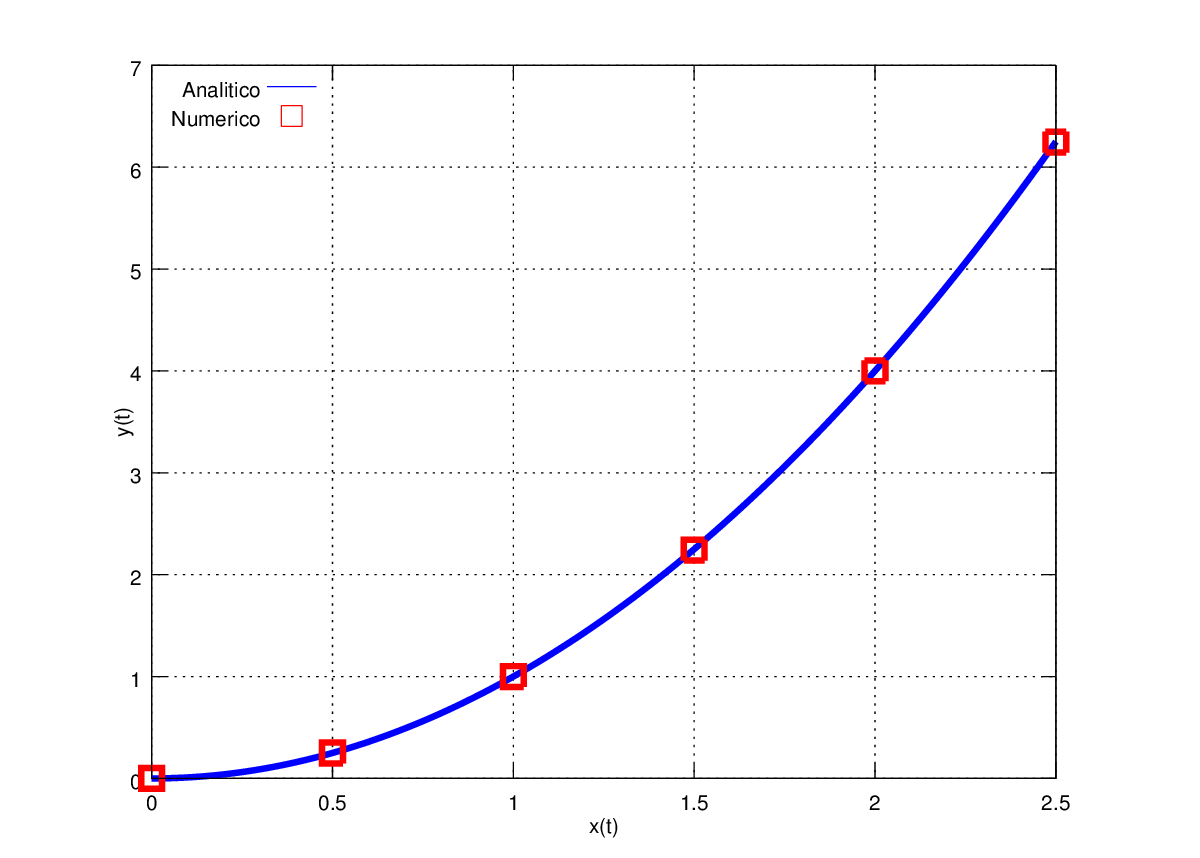
\includegraphics[width=.8\textwidth]{imagenes/chap4/x_vs_y}
\caption{Leyenda de figura.}
\end{figure}
Ejemplo de ecuación:
\begin{equation}
y(x)=x^2
\end{equation}
 % Se carga el capítulo 04
  \chapter{Consideraciones finales}

En este capítulo se sintetizan las posturas expuestas en el capítulo anterior. Se retoma la pregunta de investigación y se expresa si los resultados apoyan o no la hipótesis planteada. 

Además, se pueden hacer contribuciones teóricas o metodológicas a la disciplina y recomendaciones para trabajos futuros o para profundizar en el campo, plantear nuevas interrogantes o proponer explicaciones \textit{post hoc}. En algunos trabajos este capítulo se subdivide en otras secciones que presentan algunos de los contenidos mencionados. 
En algunas tradiciones académicas este capítulo recibe distintas denominaciones: \textit{Conclusiones}, \textit{Conclusiones y trabajos a futuro}, \textit{Consideraciones finales y recomendaciones}. 

 % Se carga el capítulo 05
 % Seguir copiando la linea de arriba para agregar más capítulos.

  \backmatter % Comando que generalos apéndices, anexos y bibliografía. NO COMENTAR

  \bibliography{bibliografia/tesis,bibliografia/ambicycle} % Agregar la cantidad de archivos .bib que se tengan para la bibliografía.
  \bibend % No comentar
  % 
  \glosario 		         % Glosario, NO comentar
  %
  \apenarabicnumbering
  \apenmatter				 % Apéndices, NO comentar
  \chapter{Datos procesados}


  \chapter{Imágenes remasterizadas}\label{Ape2}

  \chapter{Entrevistas desgrabadas}\label{Ape3}


  % Seguir copiando la linea de arriba para agregar más apéndices.
  %
  \anexarabicnumbering
  \anexmatter				 % Anexos, NO comentar
%  \chapter{Material legislativo}\label{Ane1}

XXXXX
  % Seguir copiando la linea de arriba para agregar más anexos.
  % 
\end{document}

% ===== FIN DEL DOCUMENTO =====
